\section{Motivation}
\begin{frame}[c]{Motivation}
\begin{tcolorbox}[colback=TUMBlueLighter,title=\dom]
    \begin{tabularx}{1.0\textwidth}{>{\hsize=0.30\hsize}X>{\hsize=0.8\hsize}X}
        \textbf{Input} & Graph $G = (V, E)$, $k \in \mathbb{N}$\\
        \textbf{Question} & Is there a set {$D \subseteq V$} of size at most $k$ such that ${N[D] = V}$? \\
    \end{tabularx}
\end{tcolorbox}

\begin{itemize}
\item The domination number is the minimum cardinality of a ds of $G$, denotes as $\gamma(G)$
\item \textbf{Observation:} In connected $G$ every $v\in D$ has another $z \in D$ with $d(v,z) \leq 3$.
\end{itemize}

\end{frame}

\begin{frame}[c]{Motivation}
\begin{tcolorbox}[colback=TUMBlueLighter,title=\tdom]
    \begin{tabularx}{1.0\textwidth}{>{\hsize=0.30\hsize}X>{\hsize=0.8\hsize}X}
        \textbf{Input} & Graph $G = (V, E)$, $k \in \mathbb{N}$\\
        \textbf{Question} & Is there a set $D \subseteq V$ of size at most $k$ such that for all $d_1 \in X$ exists $d_2 \in X \setminus \{d_1\}$ s.t. ${d(d_1, d_2) \leq 1}$? \\
    \end{tabularx}
\end{tcolorbox}

\begin{itemize}
    \item The total domination number is the minimum cardinality of a tds of $G$, denoted as $\gamma_t(G)$.
\end{itemize}

\end{frame}

\begin{frame}[c]{Motivation}
\begin{tcolorbox}[colback=TUMBlueLighter,title=\sdom]
    \begin{tabularx}{1.0\textwidth}{>{\hsize=0.30\hsize}X>{\hsize=0.8\hsize}X}
        \textbf{Input}    & Graph $G = (V, E)$, $k \in \mathbb{N}$\\
    \textbf{Question} & Is there a subset $D \subseteq V$ with $|D| \leq k$ such that ${N[D] = V}$ and for all $d_1 \in X$ there exists another $d_2 \in X$ such that ${d(d_1, d_2) \leq 2}$?
    \end{tabularx}
\end{tcolorbox}

\begin{itemize}
    \item The semitotal dominatinon number is the minimum cardinality of a sds of $G$, denoted as $\gamma_{2t}(G)$.
    \item \textbf{Observation}: $\gamma(G) \leq  \mathbf{\gamma_{2t}(G)}  \leq \gamma{t}(G)$
\end{itemize}
\end{frame}

\begin{frame}[c]{Example: $\gamma(G) < \mathbf{\gamma_{2t}(G)} < \gamma_t(G)$}
\begin{figure}[!ht]
    \resizebox{0.95\textwidth}{!}{
         \tikzfig{../thesis/fig/tikz/ds-examples}
    }
    \end{figure}
\end{frame}


\section{Theory}
\begin{frame}[c]{Parameterized Complexity}
    \begin{itemize}
        \item Developed by Downey and Fellows \\
        \item \textbf{Idea:~} Limit combinatorial explosion to some aspect of the problem\\
        \item 
    \end{itemize}

\end{frame}

\begin{frame}[c]{Fixed-parameter tractability}

\end{frame}

\begin{frame}[c]{Kernelization}
\begin{itemize}
    \item \textbf{Idea: } Preprocess an instance using \textit{Reduction Rules} until hard \textit{kernel} is found.
\end{itemize}

\begin{figure}
\centering
\resizebox{0.35\textwidth}{!} {
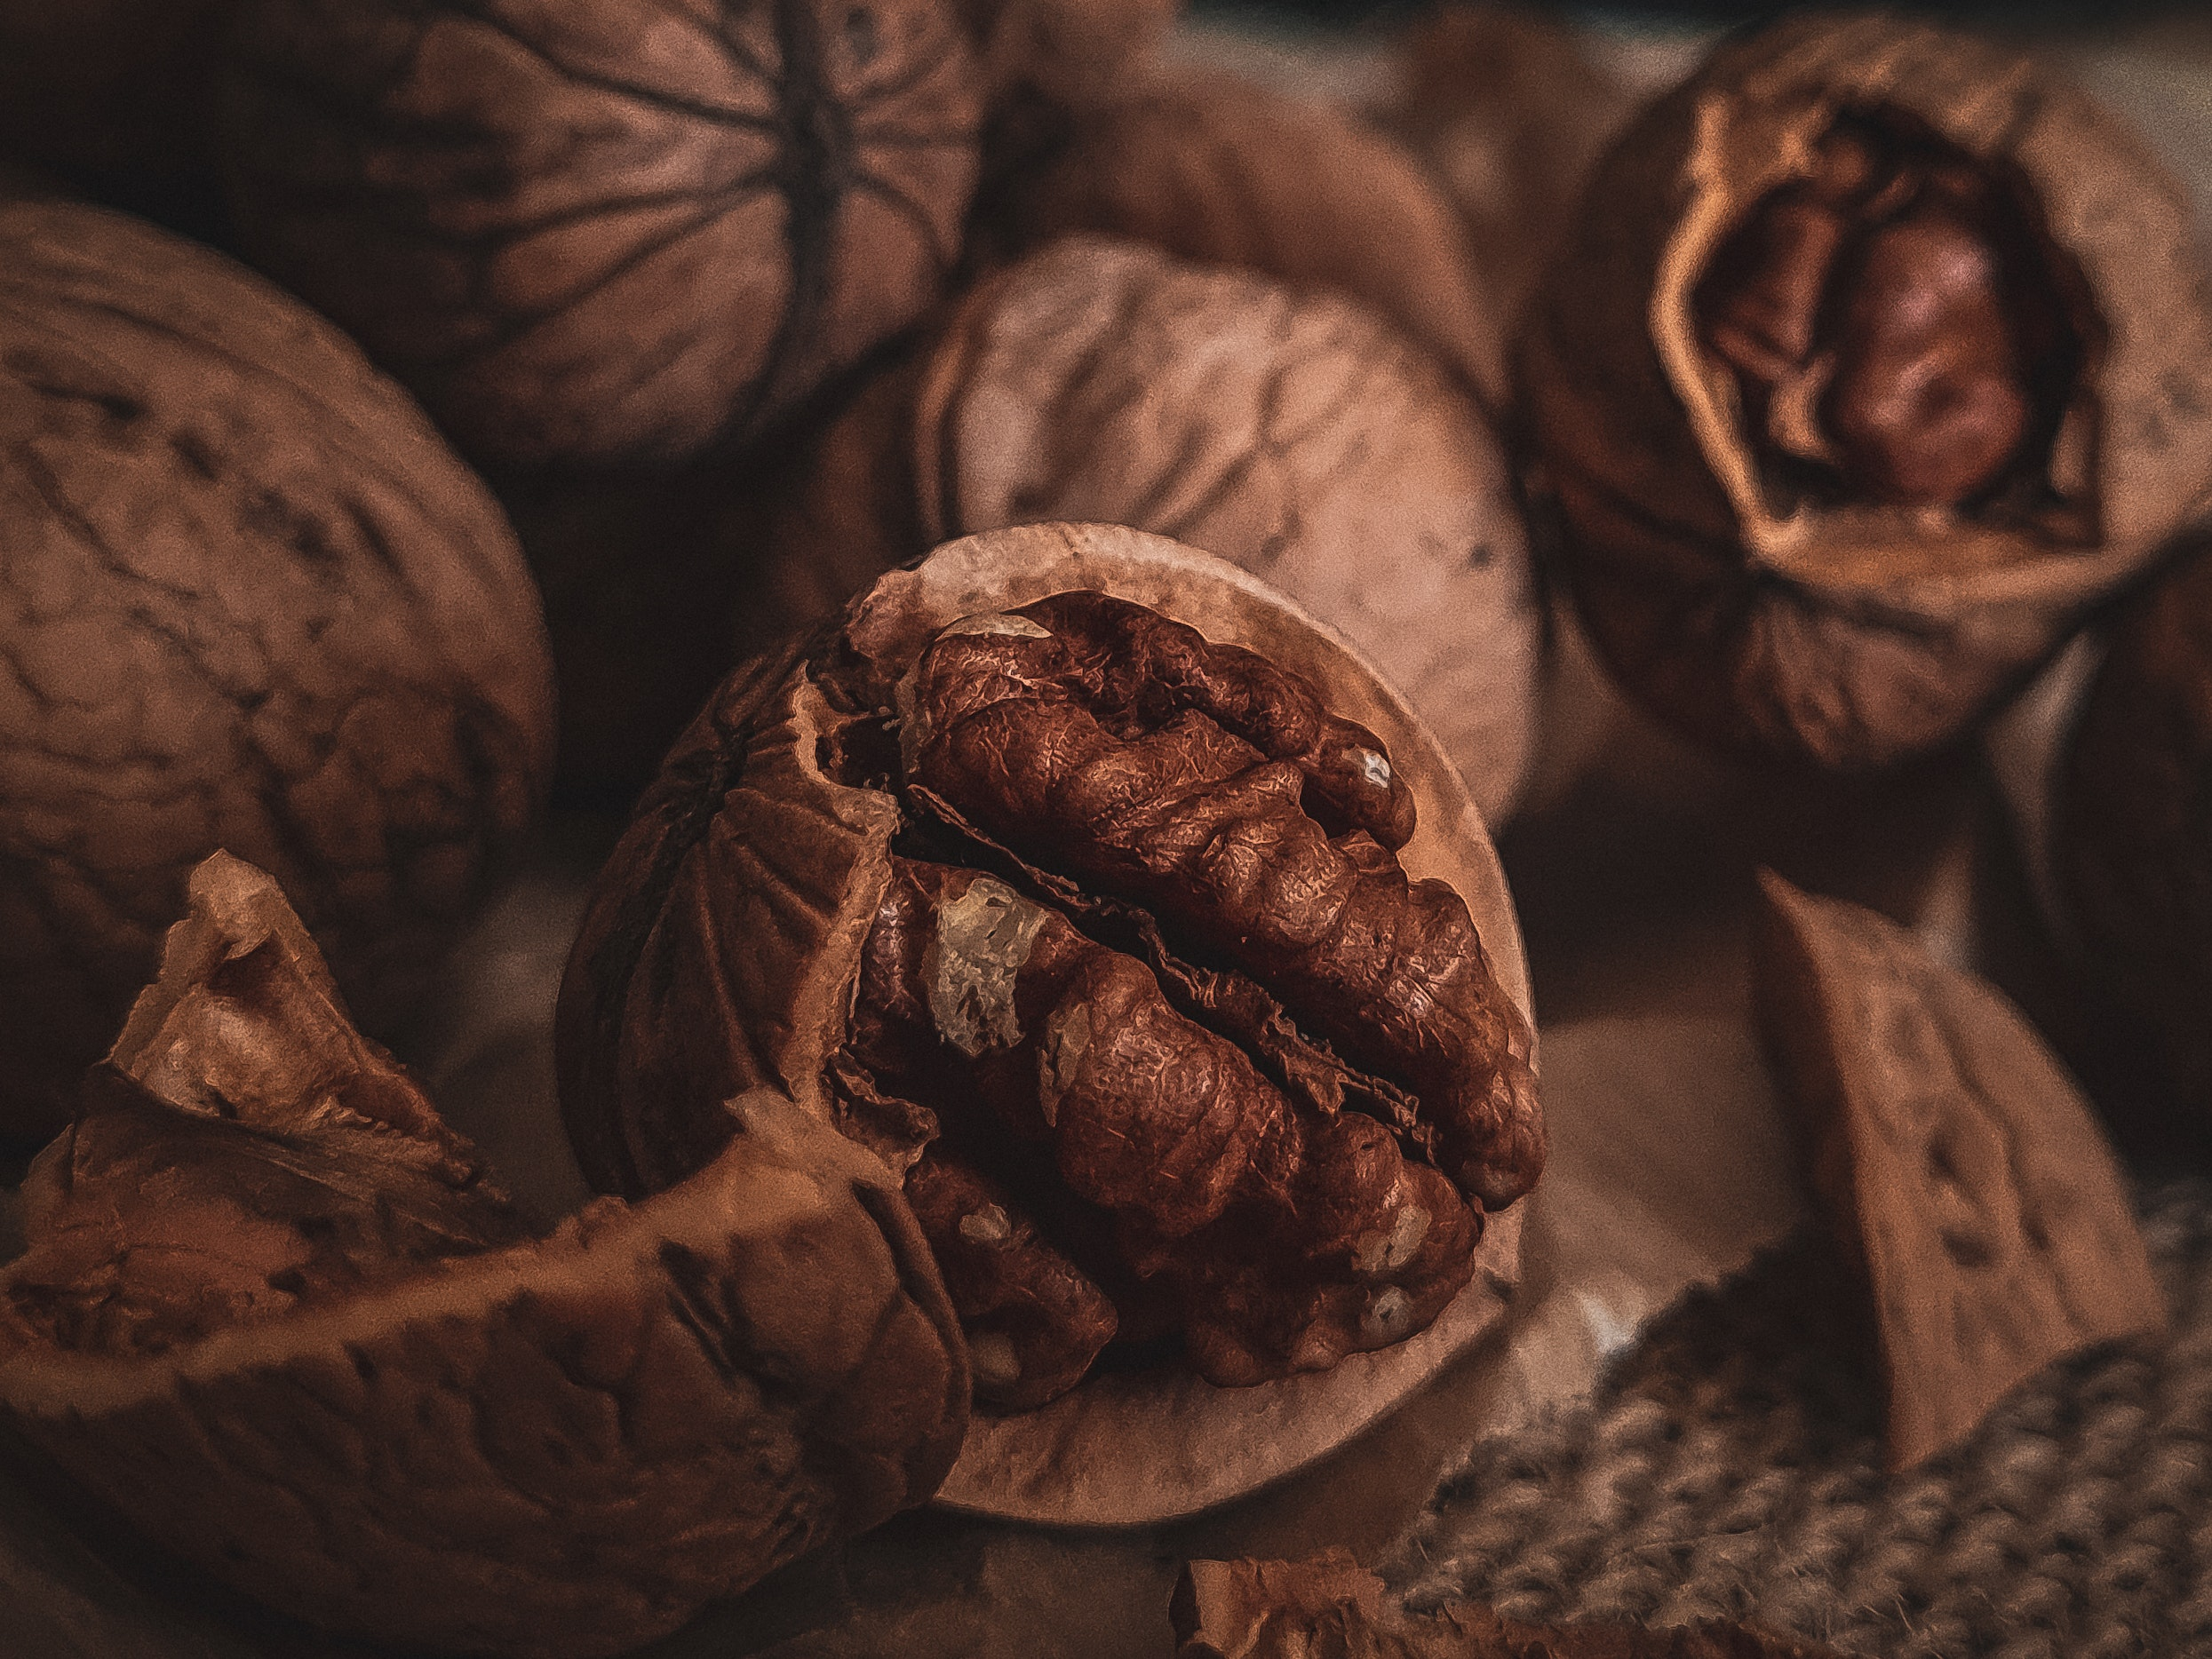
\includegraphics{fig/pexels-yulia-ilina-10400351.jpg}
}
\end{figure}
\end{frame}


\begin{frame}[c]{Kernelization}
% Moreover, we require that $size_{\mathfrak{A}}(k) \leq g(k)$ for some computable function $g:\mathbb{N} \rightarrow \mathbb{N}$.


% \item A \textit{kernelization algorithm} or \textit{kernel} is an algorithm $\mathfrak{A}$ for a parameterized problem $Q$ that given an instance $(I,k)$ of $Q$ runs in polynomial time and returns an equivalent instance $(I', k')$ of $Q$. 
% A \underline{reduction rule} is a function $\phi:\Sigma^* \times \mathbb{N} \rightarrow \Sigma^* \times \mathbb{N}$ that maps an instance $(x,k)$ to an equivalent instance $(x',k')$ such that $\phi$ is computable in time polynomial in $\abs{x}$ and $k$.
%A reduction rule is \underline{sound} (or \underline{safe}) if $(I, k) \in Q \Leftrightarrow (I',k') \in Q$.

\begin{itemize}
    \item \textbf{Idea: } Preprocess an instance using \textit{Reduction Rules} until hard \textit{kernel} is found.
\end{itemize}

\begin{figure}
\centering
\resizebox{0.7\textwidth}{!}{
    
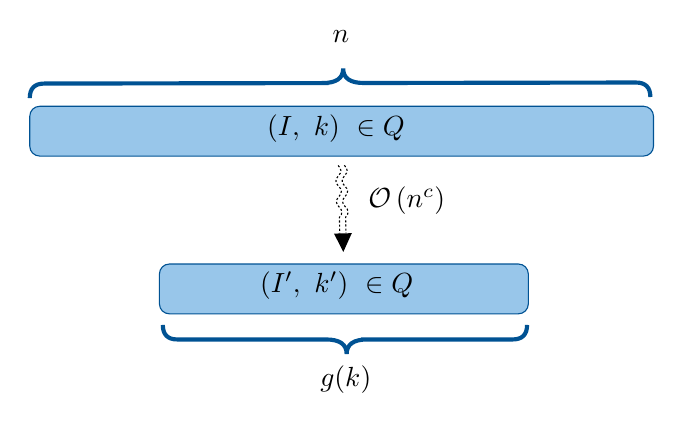
\begin{tikzpicture}[x=0.75pt,y=0.75pt,yscale=-1,xscale=1]
%uncomment if require: \path (0,290); %set diagram left start at 0, and has height of 290
\tikzset{every picture/.style={line width=0.75pt}} %set default line width to 0.75pt        

%Rounded Rect [id:dp2256907851376615] 
\draw  [color={rgb, 255:red, 0; green, 82; blue, 147 }  ,draw opacity=1 ][fill={rgb, 255:red, 152; green, 198; blue, 234 }  ,fill opacity=1 ] (129.8,74.8) .. controls (129.8,72.15) and (131.95,70) .. (134.6,70) -- (425.5,70) .. controls (428.15,70) and (430.3,72.15) .. (430.3,74.8) -- (430.3,89.2) .. controls (430.3,91.85) and (428.15,94) .. (425.5,94) -- (134.6,94) .. controls (131.95,94) and (129.8,91.85) .. (129.8,89.2) -- cycle ;
%Straight Lines [id:da34735862747158275] 
\draw  [dash pattern={on 0.75pt off 0.75pt}]  (281.37,98.46) .. controls (283.08,100.09) and (283.12,101.75) .. (281.49,103.46) .. controls (279.86,105.17) and (279.9,106.83) .. (281.61,108.46) .. controls (283.32,110.09) and (283.36,111.75) .. (281.73,113.46) .. controls (280.1,115.17) and (280.14,116.83) .. (281.85,118.46) .. controls (283.56,120.09) and (283.6,121.75) .. (281.97,123.46) -- (282.08,128.13) -- (282.15,131.13)(278.37,98.54) .. controls (280.08,100.16) and (280.12,101.82) .. (278.49,103.53) .. controls (276.86,105.24) and (276.9,106.9) .. (278.61,108.53) .. controls (280.32,110.16) and (280.36,111.82) .. (278.73,113.53) .. controls (277.1,115.24) and (277.14,116.9) .. (278.85,118.53) .. controls (280.56,120.16) and (280.6,121.82) .. (278.97,123.53) -- (279.08,128.21) -- (279.15,131.21) ;
\draw [shift={(280.87,140.17)}, rotate = 268.63] [fill={rgb, 255:red, 0; green, 0; blue, 0 }  ][line width=0.08]  [draw opacity=0] (8.93,-4.29) -- (0,0) -- (8.93,4.29) -- cycle    ;
%Rounded Rect [id:dp11606859634007116] 
\draw  [color={rgb, 255:red, 0; green, 82; blue, 147 }  ,draw opacity=1 ][fill={rgb, 255:red, 152; green, 198; blue, 234 }  ,fill opacity=1 ] (192.27,150.8) .. controls (192.27,148.15) and (194.42,146) .. (197.07,146) -- (365.2,146) .. controls (367.85,146) and (370,148.15) .. (370,150.8) -- (370,165.2) .. controls (370,167.85) and (367.85,170) .. (365.2,170) -- (197.07,170) .. controls (194.42,170) and (192.27,167.85) .. (192.27,165.2) -- cycle ;
%Shape: Brace [id:dp49500678764931805] 
\draw  [color={rgb, 255:red, 0; green, 82; blue, 147 }  ,draw opacity=1 ][line width=1.5]  (428.8,65.55) .. controls (428.79,60.88) and (426.46,58.55) .. (421.79,58.56) -- (290.81,58.79) .. controls (284.14,58.8) and (280.81,56.48) .. (280.8,51.81) .. controls (280.81,56.48) and (277.48,58.82) .. (270.81,58.83)(273.81,58.82) -- (136.79,59.06) .. controls (132.12,59.07) and (129.79,61.4) .. (129.8,66.07) ;
%Shape: Brace [id:dp39979872340961986] 
\draw  [color={rgb, 255:red, 0; green, 82; blue, 147 }  ,draw opacity=1 ][line width=1.5]  (193.9,175.35) .. controls (193.9,180.02) and (196.23,182.35) .. (200.9,182.35) -- (272.47,182.35) .. controls (279.14,182.35) and (282.47,184.68) .. (282.47,189.35) .. controls (282.47,184.68) and (285.8,182.35) .. (292.47,182.35)(289.47,182.35) -- (362.4,182.35) .. controls (367.07,182.35) and (369.4,180.02) .. (369.4,175.35) ;

% Text Node
\draw (242.9,72.9) node [anchor=north west][inner sep=0.75pt]    {$( I,\ k) \ \in Q$};
% Text Node
\draw (291.67,107.4) node [anchor=north west][inner sep=0.75pt]    {$\mathcal{O}\left( n^{c}\right)$};
% Text Node
\draw (239.5,148.4) node [anchor=north west][inner sep=0.75pt]    {$( I',\ k') \ \in Q$};
% Text Node
\draw (268.5,193.9) node [anchor=north west][inner sep=0.75pt]    {$g( k)$};
% Text Node
\draw (274.5,32.4) node [anchor=north west][inner sep=0.75pt]    {$n$};


\end{tikzpicture}

}
\end{figure}
\end{frame}


\begin{frame}[c]{Complexity Status}
 \begin{figure}
    \centering
    \resizebox{0.9\textwidth}{!}{
        

\tikzset{every picture/.style={line width=0.75pt}} %set default line width to 0.75pt        

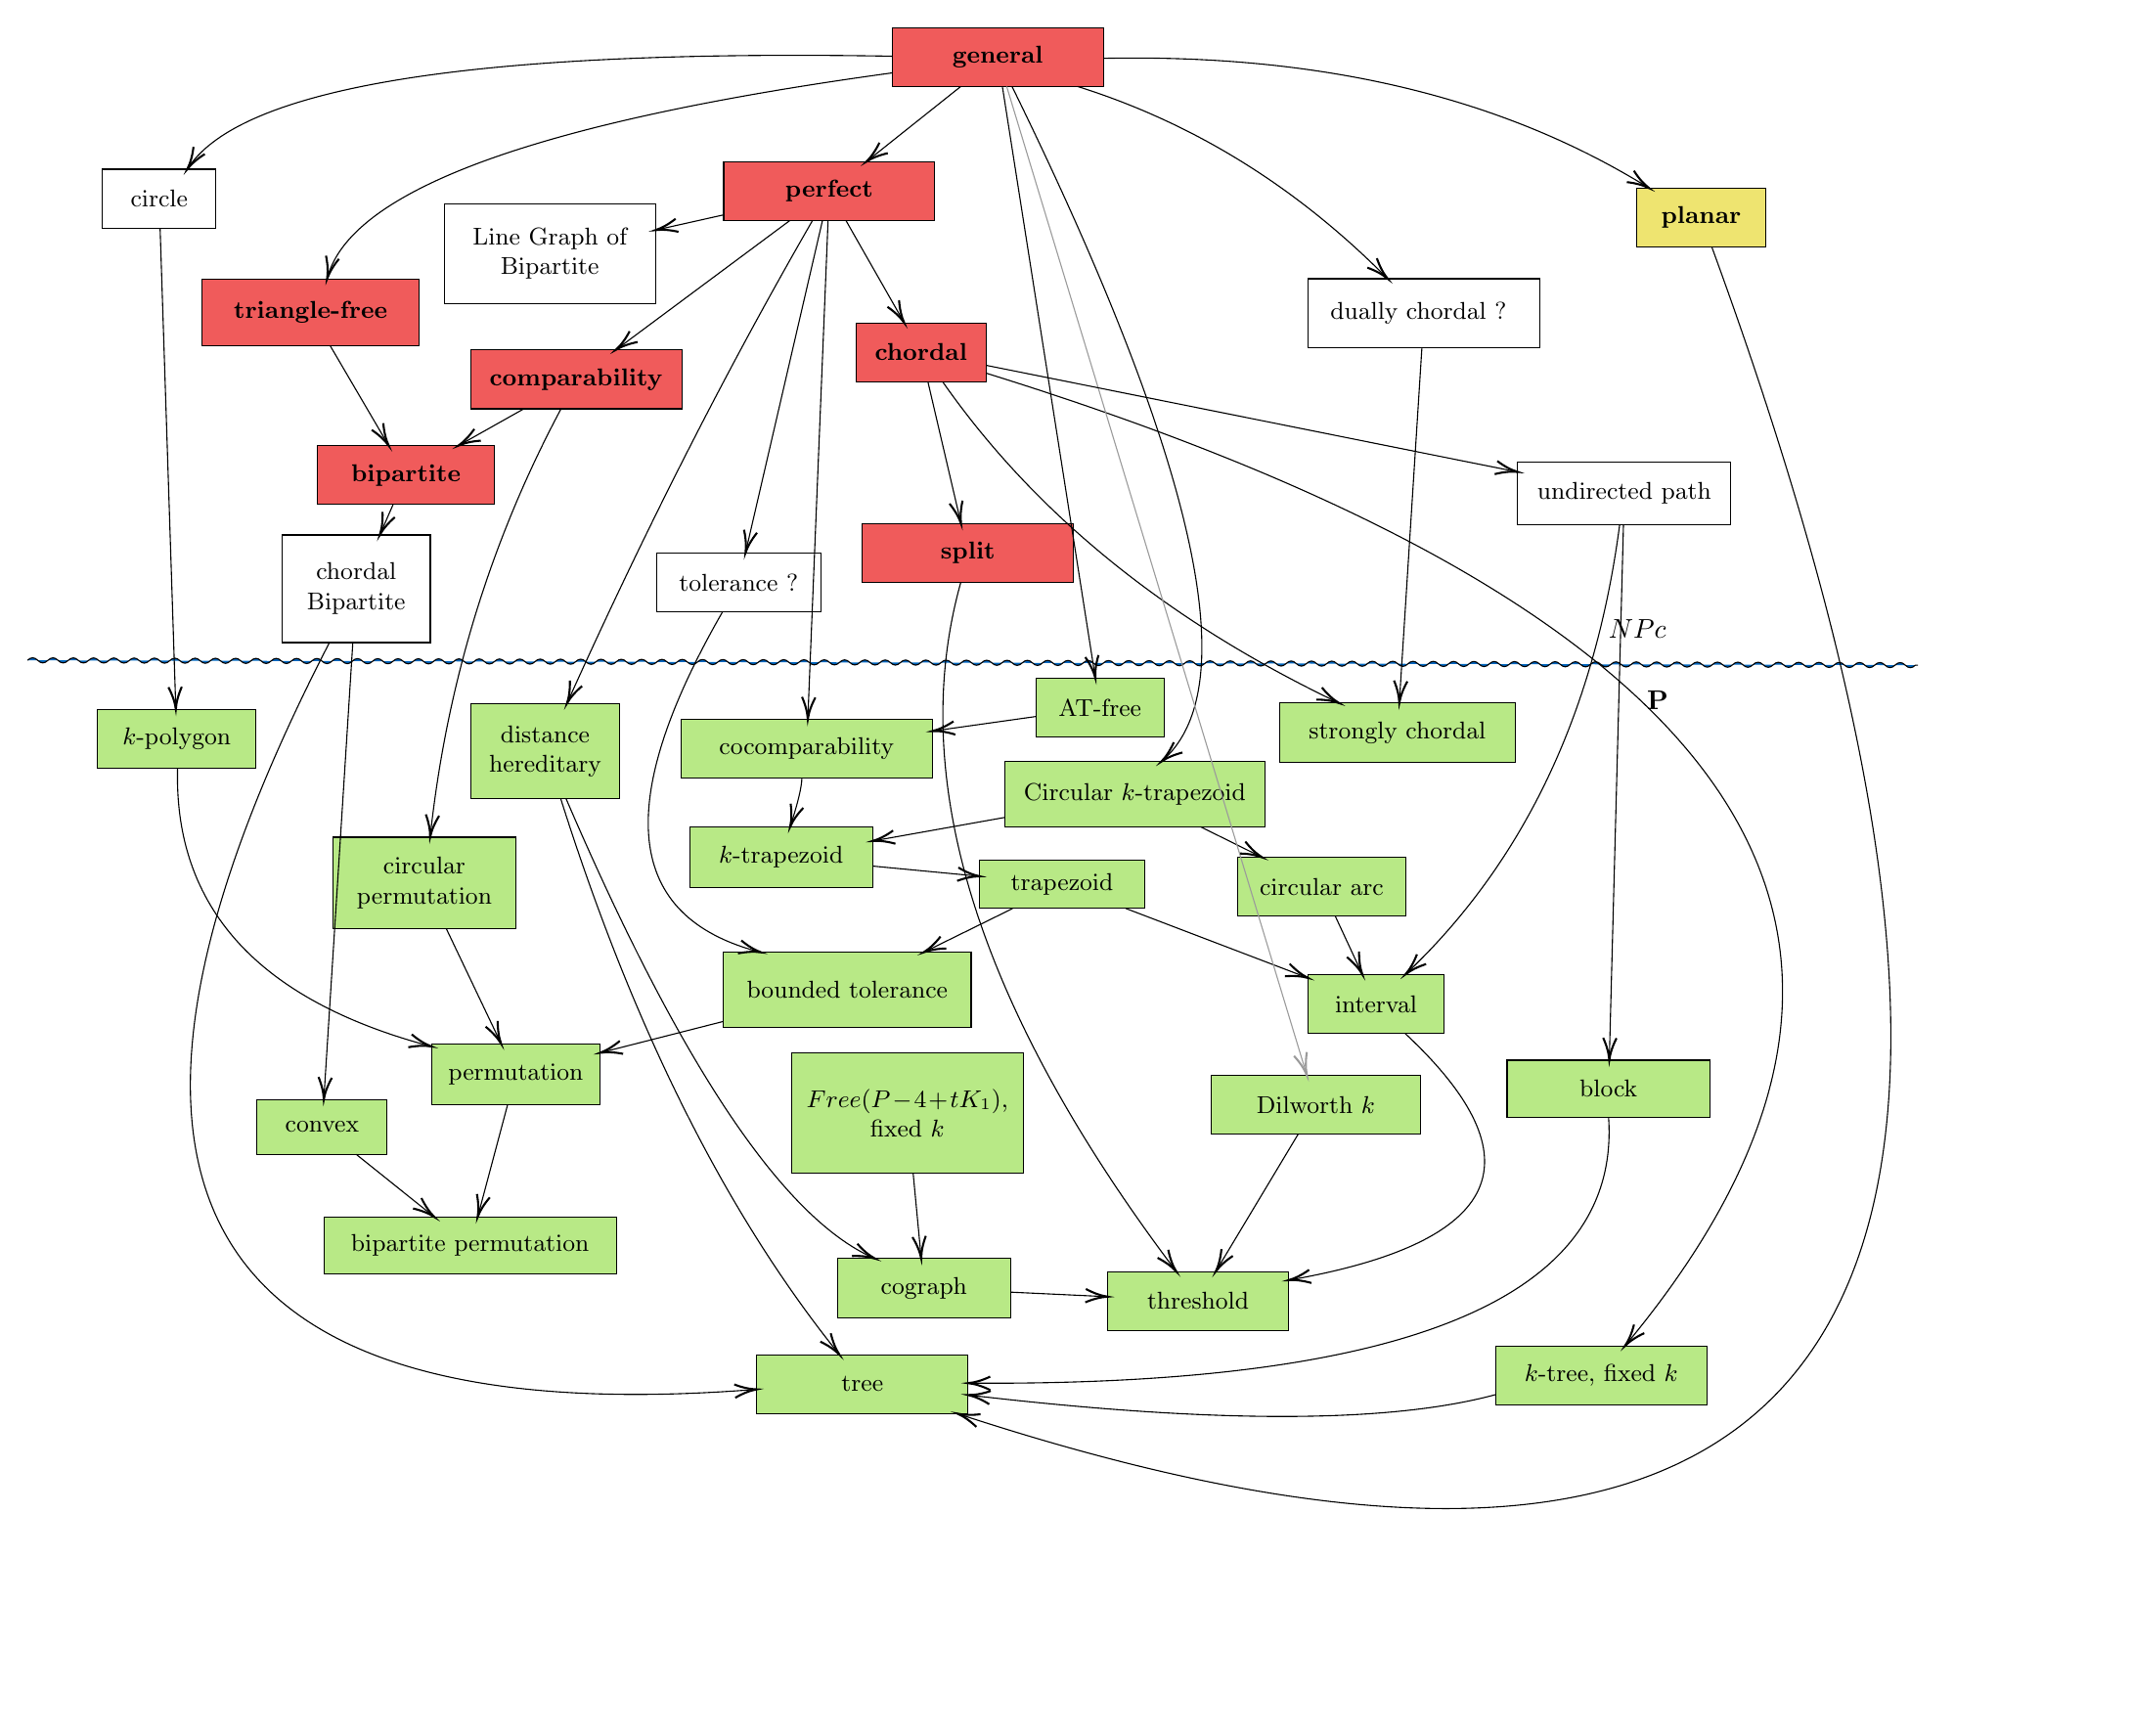
\begin{tikzpicture}[x=0.75pt,y=0.75pt,yscale=-1,xscale=1]
%uncomment if require: \path (0,617); %set diagram left start at 0, and has height of 617

%Straight Lines [id:da6521298779049807] 
\draw [fill={rgb, 255:red, 0; green, 101; blue, 189 }  ,fill opacity=1 ]   (-114.6,212.17) .. controls (-112.93,210.51) and (-111.26,210.52) .. (-109.6,212.19) .. controls (-107.93,213.86) and (-106.27,213.86) .. (-104.6,212.2) .. controls (-102.93,210.54) and (-101.27,210.54) .. (-99.6,212.21) .. controls (-97.94,213.88) and (-96.27,213.89) .. (-94.6,212.23) .. controls (-92.93,210.57) and (-91.27,210.57) .. (-89.6,212.24) .. controls (-87.93,213.91) and (-86.27,213.91) .. (-84.6,212.25) .. controls (-82.93,210.59) and (-81.26,210.6) .. (-79.6,212.27) .. controls (-77.93,213.94) and (-76.27,213.94) .. (-74.6,212.28) .. controls (-72.93,210.62) and (-71.27,210.62) .. (-69.6,212.29) .. controls (-67.93,213.96) and (-66.27,213.96) .. (-64.6,212.3) .. controls (-62.93,210.64) and (-61.26,210.65) .. (-59.6,212.32) .. controls (-57.93,213.99) and (-56.27,213.99) .. (-54.6,212.33) .. controls (-52.93,210.67) and (-51.27,210.67) .. (-49.6,212.34) .. controls (-47.94,214.01) and (-46.27,214.02) .. (-44.6,212.36) .. controls (-42.93,210.7) and (-41.27,210.7) .. (-39.6,212.37) .. controls (-37.93,214.04) and (-36.27,214.04) .. (-34.6,212.38) .. controls (-32.93,210.72) and (-31.27,210.72) .. (-29.6,212.39) .. controls (-27.94,214.06) and (-26.27,214.07) .. (-24.6,212.41) .. controls (-22.93,210.75) and (-21.27,210.75) .. (-19.6,212.42) .. controls (-17.93,214.09) and (-16.27,214.09) .. (-14.6,212.43) .. controls (-12.93,210.77) and (-11.26,210.78) .. (-9.6,212.45) .. controls (-7.93,214.12) and (-6.27,214.12) .. (-4.6,212.46) .. controls (-2.93,210.8) and (-1.27,210.8) .. (0.4,212.47) .. controls (2.07,214.14) and (3.73,214.14) .. (5.4,212.48) .. controls (7.07,210.82) and (8.74,210.83) .. (10.4,212.5) .. controls (12.07,214.17) and (13.73,214.17) .. (15.4,212.51) .. controls (17.07,210.85) and (18.73,210.85) .. (20.4,212.52) .. controls (22.06,214.19) and (23.73,214.2) .. (25.4,212.54) .. controls (27.07,210.88) and (28.73,210.88) .. (30.4,212.55) .. controls (32.07,214.22) and (33.73,214.22) .. (35.4,212.56) .. controls (37.07,210.9) and (38.73,210.9) .. (40.4,212.57) .. controls (42.06,214.24) and (43.73,214.25) .. (45.4,212.59) .. controls (47.07,210.93) and (48.73,210.93) .. (50.4,212.6) .. controls (52.07,214.27) and (53.73,214.27) .. (55.4,212.61) .. controls (57.07,210.95) and (58.74,210.96) .. (60.4,212.63) .. controls (62.07,214.3) and (63.73,214.3) .. (65.4,212.64) .. controls (67.07,210.98) and (68.73,210.98) .. (70.4,212.65) .. controls (72.07,214.32) and (73.73,214.32) .. (75.4,212.66) .. controls (77.07,211) and (78.74,211.01) .. (80.4,212.68) .. controls (82.07,214.35) and (83.73,214.35) .. (85.4,212.69) .. controls (87.07,211.03) and (88.73,211.03) .. (90.4,212.7) .. controls (92.06,214.37) and (93.73,214.38) .. (95.4,212.72) .. controls (97.07,211.06) and (98.73,211.06) .. (100.4,212.73) .. controls (102.07,214.4) and (103.73,214.4) .. (105.4,212.74) .. controls (107.07,211.08) and (108.73,211.08) .. (110.4,212.75) .. controls (112.06,214.42) and (113.73,214.43) .. (115.4,212.77) .. controls (117.07,211.11) and (118.73,211.11) .. (120.4,212.78) .. controls (122.07,214.45) and (123.73,214.45) .. (125.4,212.79) .. controls (127.07,211.13) and (128.74,211.14) .. (130.4,212.81) .. controls (132.07,214.48) and (133.73,214.48) .. (135.4,212.82) .. controls (137.07,211.16) and (138.73,211.16) .. (140.4,212.83) .. controls (142.06,214.5) and (143.73,214.51) .. (145.4,212.85) .. controls (147.07,211.19) and (148.73,211.19) .. (150.4,212.86) .. controls (152.07,214.53) and (153.73,214.53) .. (155.4,212.87) .. controls (157.07,211.21) and (158.73,211.21) .. (160.4,212.88) .. controls (162.06,214.55) and (163.73,214.56) .. (165.4,212.9) .. controls (167.07,211.24) and (168.73,211.24) .. (170.4,212.91) .. controls (172.07,214.58) and (173.73,214.58) .. (175.4,212.92) .. controls (177.07,211.26) and (178.74,211.27) .. (180.4,212.94) .. controls (182.07,214.61) and (183.73,214.61) .. (185.4,212.95) .. controls (187.07,211.29) and (188.73,211.29) .. (190.4,212.96) .. controls (192.07,214.63) and (193.73,214.63) .. (195.4,212.97) .. controls (197.07,211.31) and (198.74,211.32) .. (200.4,212.99) .. controls (202.07,214.66) and (203.73,214.66) .. (205.4,213) .. controls (207.07,211.34) and (208.73,211.34) .. (210.4,213.01) .. controls (212.06,214.68) and (213.73,214.69) .. (215.4,213.03) .. controls (217.07,211.37) and (218.73,211.37) .. (220.4,213.04) .. controls (222.07,214.71) and (223.73,214.71) .. (225.4,213.05) .. controls (227.07,211.39) and (228.73,211.39) .. (230.4,213.06) .. controls (232.06,214.73) and (233.73,214.74) .. (235.4,213.08) .. controls (237.07,211.42) and (238.73,211.42) .. (240.4,213.09) .. controls (242.07,214.76) and (243.73,214.76) .. (245.4,213.1) .. controls (247.07,211.44) and (248.74,211.45) .. (250.4,213.12) .. controls (252.07,214.79) and (253.73,214.79) .. (255.4,213.13) .. controls (257.07,211.47) and (258.73,211.47) .. (260.4,213.14) .. controls (262.07,214.81) and (263.73,214.81) .. (265.4,213.15) .. controls (267.07,211.49) and (268.74,211.5) .. (270.4,213.17) .. controls (272.07,214.84) and (273.73,214.84) .. (275.4,213.18) .. controls (277.07,211.52) and (278.73,211.52) .. (280.4,213.19) .. controls (282.06,214.86) and (283.73,214.87) .. (285.4,213.21) .. controls (287.07,211.55) and (288.73,211.55) .. (290.4,213.22) .. controls (292.07,214.89) and (293.73,214.89) .. (295.4,213.23) .. controls (297.07,211.57) and (298.73,211.57) .. (300.4,213.24) .. controls (302.06,214.91) and (303.73,214.92) .. (305.4,213.26) .. controls (307.07,211.6) and (308.73,211.6) .. (310.4,213.27) .. controls (312.07,214.94) and (313.73,214.94) .. (315.4,213.28) .. controls (317.07,211.62) and (318.74,211.63) .. (320.4,213.3) .. controls (322.07,214.97) and (323.73,214.97) .. (325.4,213.31) .. controls (327.07,211.65) and (328.73,211.65) .. (330.4,213.32) .. controls (332.07,214.99) and (333.73,214.99) .. (335.4,213.33) .. controls (337.07,211.67) and (338.74,211.68) .. (340.4,213.35) .. controls (342.07,215.02) and (343.73,215.02) .. (345.4,213.36) .. controls (347.07,211.7) and (348.73,211.7) .. (350.4,213.37) .. controls (352.06,215.04) and (353.73,215.05) .. (355.4,213.39) .. controls (357.07,211.73) and (358.73,211.73) .. (360.4,213.4) .. controls (362.07,215.07) and (363.73,215.07) .. (365.4,213.41) .. controls (367.07,211.75) and (368.73,211.75) .. (370.4,213.42) .. controls (372.06,215.09) and (373.73,215.1) .. (375.4,213.44) .. controls (377.07,211.78) and (378.73,211.78) .. (380.4,213.45) .. controls (382.07,215.12) and (383.73,215.12) .. (385.4,213.46) .. controls (387.07,211.8) and (388.74,211.81) .. (390.4,213.48) .. controls (392.07,215.15) and (393.73,215.15) .. (395.4,213.49) .. controls (397.07,211.83) and (398.73,211.83) .. (400.4,213.5) .. controls (402.06,215.17) and (403.73,215.18) .. (405.4,213.52) .. controls (407.07,211.86) and (408.73,211.86) .. (410.4,213.53) .. controls (412.07,215.2) and (413.73,215.2) .. (415.4,213.54) .. controls (417.07,211.88) and (418.73,211.88) .. (420.4,213.55) .. controls (422.06,215.22) and (423.73,215.23) .. (425.4,213.57) .. controls (427.07,211.91) and (428.73,211.91) .. (430.4,213.58) .. controls (432.07,215.25) and (433.73,215.25) .. (435.4,213.59) .. controls (437.07,211.93) and (438.74,211.94) .. (440.4,213.61) .. controls (442.07,215.28) and (443.73,215.28) .. (445.4,213.62) .. controls (447.07,211.96) and (448.73,211.96) .. (450.4,213.63) .. controls (452.07,215.3) and (453.73,215.3) .. (455.4,213.64) .. controls (457.07,211.98) and (458.74,211.99) .. (460.4,213.66) .. controls (462.07,215.33) and (463.73,215.33) .. (465.4,213.67) .. controls (467.07,212.01) and (468.73,212.01) .. (470.4,213.68) .. controls (472.06,215.35) and (473.73,215.36) .. (475.4,213.7) .. controls (477.07,212.04) and (478.73,212.04) .. (480.4,213.71) .. controls (482.07,215.38) and (483.73,215.38) .. (485.4,213.72) .. controls (487.07,212.06) and (488.73,212.06) .. (490.4,213.73) .. controls (492.06,215.4) and (493.73,215.41) .. (495.4,213.75) .. controls (497.07,212.09) and (498.73,212.09) .. (500.4,213.76) .. controls (502.07,215.43) and (503.73,215.43) .. (505.4,213.77) .. controls (507.07,212.11) and (508.74,212.12) .. (510.4,213.79) .. controls (512.07,215.46) and (513.73,215.46) .. (515.4,213.8) .. controls (517.07,212.14) and (518.73,212.14) .. (520.4,213.81) .. controls (522.07,215.48) and (523.73,215.48) .. (525.4,213.82) .. controls (527.07,212.16) and (528.74,212.17) .. (530.4,213.84) .. controls (532.07,215.51) and (533.73,215.51) .. (535.4,213.85) .. controls (537.07,212.19) and (538.73,212.19) .. (540.4,213.86) .. controls (542.06,215.53) and (543.73,215.54) .. (545.4,213.88) .. controls (547.07,212.22) and (548.73,212.22) .. (550.4,213.89) .. controls (552.07,215.56) and (553.73,215.56) .. (555.4,213.9) .. controls (557.07,212.24) and (558.73,212.24) .. (560.4,213.91) .. controls (562.06,215.58) and (563.73,215.59) .. (565.4,213.93) .. controls (567.07,212.27) and (568.73,212.27) .. (570.4,213.94) .. controls (572.07,215.61) and (573.73,215.61) .. (575.4,213.95) .. controls (577.07,212.29) and (578.74,212.3) .. (580.4,213.97) .. controls (582.07,215.64) and (583.73,215.64) .. (585.4,213.98) .. controls (587.07,212.32) and (588.73,212.32) .. (590.4,213.99) .. controls (592.07,215.66) and (593.73,215.66) .. (595.4,214) .. controls (597.07,212.34) and (598.74,212.35) .. (600.4,214.02) .. controls (602.07,215.69) and (603.73,215.69) .. (605.4,214.03) .. controls (607.07,212.37) and (608.73,212.37) .. (610.4,214.04) .. controls (612.06,215.71) and (613.73,215.72) .. (615.4,214.06) .. controls (617.07,212.4) and (618.73,212.4) .. (620.4,214.07) .. controls (622.07,215.74) and (623.73,215.74) .. (625.4,214.08) .. controls (627.07,212.42) and (628.74,212.43) .. (630.4,214.1) .. controls (632.07,215.77) and (633.73,215.77) .. (635.4,214.11) .. controls (637.07,212.45) and (638.73,212.45) .. (640.4,214.12) .. controls (642.07,215.79) and (643.73,215.79) .. (645.4,214.13) .. controls (647.07,212.47) and (648.74,212.48) .. (650.4,214.15) .. controls (652.07,215.82) and (653.73,215.82) .. (655.4,214.16) .. controls (657.07,212.5) and (658.73,212.5) .. (660.4,214.17) .. controls (662.06,215.84) and (663.73,215.85) .. (665.4,214.19) .. controls (667.07,212.53) and (668.73,212.53) .. (670.4,214.2) .. controls (672.07,215.87) and (673.73,215.87) .. (675.4,214.21) .. controls (677.07,212.55) and (678.73,212.55) .. (680.4,214.22) .. controls (682.06,215.89) and (683.73,215.9) .. (685.4,214.24) .. controls (687.07,212.58) and (688.73,212.58) .. (690.4,214.25) .. controls (692.07,215.92) and (693.73,215.92) .. (695.4,214.26) .. controls (697.07,212.6) and (698.74,212.61) .. (700.4,214.28) .. controls (702.07,215.95) and (703.73,215.95) .. (705.4,214.29) .. controls (707.07,212.63) and (708.73,212.63) .. (710.4,214.3) .. controls (712.07,215.97) and (713.73,215.97) .. (715.4,214.31) .. controls (717.07,212.65) and (718.74,212.66) .. (720.4,214.33) .. controls (722.07,216) and (723.73,216) .. (725.4,214.34) .. controls (727.07,212.68) and (728.73,212.68) .. (730.4,214.35) .. controls (732.06,216.02) and (733.73,216.03) .. (735.4,214.37) .. controls (737.07,212.71) and (738.73,212.71) .. (740.4,214.38) .. controls (742.07,216.05) and (743.73,216.05) .. (745.4,214.39) .. controls (747.07,212.73) and (748.73,212.73) .. (750.4,214.4) .. controls (752.06,216.07) and (753.73,216.08) .. (755.4,214.42) .. controls (757.07,212.76) and (758.73,212.76) .. (760.4,214.43) .. controls (762.07,216.1) and (763.73,216.1) .. (765.4,214.44) .. controls (767.07,212.78) and (768.74,212.79) .. (770.4,214.46) .. controls (772.07,216.13) and (773.73,216.13) .. (775.4,214.47) .. controls (777.07,212.81) and (778.73,212.81) .. (780.4,214.48) .. controls (782.07,216.15) and (783.73,216.15) .. (785.4,214.49) .. controls (787.07,212.83) and (788.74,212.84) .. (790.4,214.51) .. controls (792.07,216.18) and (793.73,216.18) .. (795.4,214.52) .. controls (797.07,212.86) and (798.73,212.86) .. (800.4,214.53) .. controls (802.06,216.2) and (803.73,216.21) .. (805.4,214.55) .. controls (807.07,212.89) and (808.73,212.89) .. (810.4,214.56) .. controls (812.07,216.23) and (813.73,216.23) .. (815.4,214.57) -- (816.6,214.57) -- (816.6,214.57) ;

% Text Node
\draw  [fill={rgb, 255:red, 233; green, 17; blue, 17 }  ,fill opacity=0.69 ]  (228.33,-33.4) -- (332.33,-33.4) -- (332.33,-4.4) -- (228.33,-4.4) -- cycle  ;
\draw (280.33,-18.9) node  [font=\small] [align=left] {\begin{minipage}[lt]{68pt}\setlength\topsep{0pt}
\begin{center}
\textbf{perfect}
\end{center}

\end{minipage}};
% Text Node
\draw    (90.67,-12.58) -- (194.67,-12.58) -- (194.67,36.42) -- (90.67,36.42) -- cycle  ;
\draw (142.67,11.92) node  [font=\small] [align=left] {\begin{minipage}[lt]{68pt}\setlength\topsep{0pt}
\begin{center}
Line Graph of Bipartite
\end{center}

\end{minipage}};
% Text Node
\draw  [fill={rgb, 255:red, 233; green, 17; blue, 17 }  ,fill opacity=0.69 ]  (103.67,59.27) -- (207.67,59.27) -- (207.67,88.27) -- (103.67,88.27) -- cycle  ;
\draw (155.67,73.77) node  [font=\small] [align=left] {\begin{minipage}[lt]{68pt}\setlength\topsep{0pt}
\begin{center}
\textbf{comparability}
\end{center}

\end{minipage}};
% Text Node
\draw    (195.2,159.27) -- (276.2,159.27) -- (276.2,188.27) -- (195.2,188.27) -- cycle  ;
\draw (235.7,173.77) node  [font=\small] [align=left] {\begin{minipage}[lt]{52.63pt}\setlength\topsep{0pt}
\begin{center}
tolerance ?
\end{center}

\end{minipage}};
% Text Node
\draw  [fill={rgb, 255:red, 184; green, 233; blue, 134 }  ,fill opacity=1 ]  (382.2,220.93) -- (445.2,220.93) -- (445.2,249.93) -- (382.2,249.93) -- cycle  ;
\draw (413.7,235.43) node  [font=\small] [align=left] {\begin{minipage}[lt]{40.39pt}\setlength\topsep{0pt}
\begin{center}
AT-free
\end{center}

\end{minipage}};
% Text Node
\draw  [fill={rgb, 255:red, 233; green, 17; blue, 17 }  ,fill opacity=0.69 ]  (293.53,45.93) -- (357.53,45.93) -- (357.53,74.93) -- (293.53,74.93) -- cycle  ;
\draw (325.53,60.43) node  [font=\small] [align=left] {\begin{minipage}[lt]{40.62pt}\setlength\topsep{0pt}
\begin{center}
\textbf{chordal}
\end{center}

\end{minipage}};
% Text Node
\draw  [fill={rgb, 255:red, 233; green, 17; blue, 17 }  ,fill opacity=0.69 ]  (296.67,144.93) -- (400.67,144.93) -- (400.67,173.93) -- (296.67,173.93) -- cycle  ;
\draw (348.67,159.43) node  [font=\small] [align=left] {\begin{minipage}[lt]{68pt}\setlength\topsep{0pt}
\begin{center}
\textbf{split}
\end{center}

\end{minipage}};
% Text Node
\draw  [fill={rgb, 255:red, 184; green, 233; blue, 134 }  ,fill opacity=1 ]  (608.67,549.93) -- (712.67,549.93) -- (712.67,578.93) -- (608.67,578.93) -- cycle  ;
\draw (660.67,564.43) node  [font=\small] [align=left] {\begin{minipage}[lt]{68pt}\setlength\topsep{0pt}
\begin{center}
$\displaystyle k$-tree, fixed $\displaystyle k$
\end{center}

\end{minipage}};
% Text Node
\draw  [color={rgb, 255:red, 0; green, 0; blue, 0 }  ,draw opacity=1 ][fill={rgb, 255:red, 184; green, 233; blue, 134 }  ,fill opacity=1 ]  (207.17,241.27) -- (331.17,241.27) -- (331.17,270.27) -- (207.17,270.27) -- cycle  ;
\draw (269.17,255.77) node  [font=\small] [align=left] {\begin{minipage}[lt]{81.83pt}\setlength\topsep{0pt}
\begin{center}
cocomparability
\end{center}

\end{minipage}};
% Text Node
\draw  [fill={rgb, 255:red, 184; green, 233; blue, 134 }  ,fill opacity=1 ]  (244.67,554.27) -- (348.67,554.27) -- (348.67,583.27) -- (244.67,583.27) -- cycle  ;
\draw (296.67,568.77) node  [font=\small] [align=left] {\begin{minipage}[lt]{68pt}\setlength\topsep{0pt}
\begin{center}
tree
\end{center}

\end{minipage}};
% Text Node
\draw    (-77.8,-29.73) -- (-21.8,-29.73) -- (-21.8,-0.73) -- (-77.8,-0.73) -- cycle  ;
\draw (-49.8,-15.23) node  [font=\small] [align=left] {\begin{minipage}[lt]{35.63pt}\setlength\topsep{0pt}
\begin{center}
circle
\end{center}

\end{minipage}};
% Text Node
\draw    (10.8,150.42) -- (83.8,150.42) -- (83.8,203.42) -- (10.8,203.42) -- cycle  ;
\draw (47.3,176.92) node  [font=\small] [align=left] {\begin{minipage}[lt]{47.1pt}\setlength\topsep{0pt}
\begin{center}
chordal Bipartite
\end{center}

\end{minipage}};
% Text Node
\draw  [fill={rgb, 255:red, 233; green, 17; blue, 17 }  ,fill opacity=0.69 ]  (28.3,106.47) -- (115.3,106.47) -- (115.3,135.47) -- (28.3,135.47) -- cycle  ;
\draw (71.8,120.97) node  [font=\small] [align=left] {\begin{minipage}[lt]{56.39pt}\setlength\topsep{0pt}
\begin{center}
\textbf{bipartite}
\end{center}

\end{minipage}};
% Text Node
\draw  [fill={rgb, 255:red, 184; green, 233; blue, 134 }  ,fill opacity=1 ]  (366.87,262.15) -- (494.87,262.15) -- (494.87,294.15) -- (366.87,294.15) -- cycle  ;
\draw (430.87,278.15) node  [font=\small] [align=left] {\begin{minipage}[lt]{84.59pt}\setlength\topsep{0pt}
\begin{center}
Circular $\displaystyle k$-trapezoid
\end{center}

\end{minipage}};
% Text Node
\draw  [fill={rgb, 255:red, 184; green, 233; blue, 134 }  ,fill opacity=1 ]  (211.6,294.24) -- (301.6,294.24) -- (301.6,324.24) -- (211.6,324.24) -- cycle  ;
\draw (256.6,309.24) node  [font=\small] [align=left] {\begin{minipage}[lt]{58.21pt}\setlength\topsep{0pt}
\begin{center}
$\displaystyle k$-trapezoid
\end{center}

\end{minipage}};
% Text Node
\draw  [fill={rgb, 255:red, 184; green, 233; blue, 134 }  ,fill opacity=1 ]  (354.53,310.45) -- (435.53,310.45) -- (435.53,334.45) -- (354.53,334.45) -- cycle  ;
\draw (395.03,322.45) node  [font=\small] [align=left] {\begin{minipage}[lt]{52.18pt}\setlength\topsep{0pt}
\begin{center}
trapezoid
\end{center}

\end{minipage}};
% Text Node
\draw  [fill={rgb, 255:red, 184; green, 233; blue, 134 }  ,fill opacity=1 ]  (228.2,356.05) -- (350.2,356.05) -- (350.2,393.05) -- (228.2,393.05) -- cycle  ;
\draw (289.2,374.55) node  [font=\small] [align=left] {\begin{minipage}[lt]{80.51pt}\setlength\topsep{0pt}
\begin{center}
bounded tolerance
\end{center}

\end{minipage}};
% Text Node
\draw  [fill={rgb, 255:red, 184; green, 233; blue, 134 }  ,fill opacity=1 ]  (84.37,401.11) -- (167.37,401.11) -- (167.37,431.11) -- (84.37,431.11) -- cycle  ;
\draw (125.87,416.11) node  [font=\small] [align=left] {\begin{minipage}[lt]{53.77pt}\setlength\topsep{0pt}
\begin{center}
permutation
\end{center}

\end{minipage}};
% Text Node
\draw  [fill={rgb, 255:red, 184; green, 233; blue, 134 }  ,fill opacity=1 ]  (31.37,486.49) -- (175.37,486.49) -- (175.37,514.49) -- (31.37,514.49) -- cycle  ;
\draw (103.37,500.49) node  [font=\small] [align=left] {\begin{minipage}[lt]{95.25pt}\setlength\topsep{0pt}
\begin{center}
bipartite permutation
\end{center}

\end{minipage}};
% Text Node
\draw  [fill={rgb, 255:red, 184; green, 233; blue, 134 }  ,fill opacity=1 ]  (-1.53,428.57) -- (62.47,428.57) -- (62.47,455.57) -- (-1.53,455.57) -- cycle  ;
\draw (30.47,442.07) node  [font=\small] [align=left] {\begin{minipage}[lt]{40.53pt}\setlength\topsep{0pt}
\begin{center}
convex
\end{center}

\end{minipage}};
% Text Node
\draw  [fill={rgb, 255:red, 184; green, 233; blue, 134 }  ,fill opacity=1 ]  (516.2,366.93) -- (583.2,366.93) -- (583.2,395.93) -- (516.2,395.93) -- cycle  ;
\draw (549.7,381.43) node  [font=\small] [align=left] {\begin{minipage}[lt]{43.11pt}\setlength\topsep{0pt}
\begin{center}
interval
\end{center}

\end{minipage}};
% Text Node
\draw  [fill={rgb, 255:red, 184; green, 233; blue, 134 }  ,fill opacity=1 ]  (417.53,513.27) -- (506.53,513.27) -- (506.53,542.27) -- (417.53,542.27) -- cycle  ;
\draw (462.03,527.77) node  [font=\small] [align=left] {\begin{minipage}[lt]{57.62pt}\setlength\topsep{0pt}
\begin{center}
threshold
\end{center}

\end{minipage}};
% Text Node
\draw  [fill={rgb, 255:red, 184; green, 233; blue, 134 }  ,fill opacity=1 ]  (468.53,416.6) -- (571.53,416.6) -- (571.53,445.6) -- (468.53,445.6) -- cycle  ;
\draw (520.03,431.1) node  [font=\small] [align=left] {\begin{minipage}[lt]{67.14pt}\setlength\topsep{0pt}
\begin{center}
Dilworth $\displaystyle k$
\end{center}

\end{minipage}};
% Text Node
\draw  [fill={rgb, 255:red, 184; green, 233; blue, 134 }  ,fill opacity=1 ]  (284.53,506.93) -- (369.53,506.93) -- (369.53,535.93) -- (284.53,535.93) -- cycle  ;
\draw (327.03,521.43) node  [font=\small] [align=left] {\begin{minipage}[lt]{55.35pt}\setlength\topsep{0pt}
\begin{center}
cograph
\end{center}

\end{minipage}};
% Text Node
\draw  [fill={rgb, 255:red, 184; green, 233; blue, 134 }  ,fill opacity=1 ]  (481.4,309.27) -- (564.4,309.27) -- (564.4,338.27) -- (481.4,338.27) -- cycle  ;
\draw (522.9,323.77) node  [font=\small] [align=left] {\begin{minipage}[lt]{53.72pt}\setlength\topsep{0pt}
\begin{center}
circular arc
\end{center}

\end{minipage}};
% Text Node
\draw  [fill={rgb, 255:red, 255; green, 255; blue, 255 }  ,fill opacity=1 ]  (516.37,24.22) -- (630.37,24.22) -- (630.37,58.22) -- (516.37,58.22) -- cycle  ;
\draw (573.37,41.22) node  [font=\small] [align=left] {\begin{minipage}[lt]{74.85pt}\setlength\topsep{0pt}
\begin{center}
dually chordal ? $ $
\end{center}

\end{minipage}};
% Text Node
\draw  [fill={rgb, 255:red, 184; green, 233; blue, 134 }  ,fill opacity=1 ]  (502.23,233.27) -- (618.23,233.27) -- (618.23,262.27) -- (502.23,262.27) -- cycle  ;
\draw (560.23,247.77) node  [font=\small] [align=left] {\begin{minipage}[lt]{76.39pt}\setlength\topsep{0pt}
\begin{center}
strongly chordal
\end{center}

\end{minipage}};
% Text Node
\draw  [fill={rgb, 255:red, 184; green, 233; blue, 134 }  ,fill opacity=1 ]  (35.9,299.3) -- (125.9,299.3) -- (125.9,344.3) -- (35.9,344.3) -- cycle  ;
\draw (80.9,321.8) node  [font=\small] [align=left] {\begin{minipage}[lt]{58.34pt}\setlength\topsep{0pt}
\begin{center}
circular permutation
\end{center}

\end{minipage}};
% Text Node
\draw  [fill={rgb, 255:red, 184; green, 233; blue, 134 }  ,fill opacity=1 ]  (-80.1,236.27) -- (-2.1,236.27) -- (-2.1,265.27) -- (-80.1,265.27) -- cycle  ;
\draw (-41.1,250.77) node  [font=\small] [align=left] {\begin{minipage}[lt]{50.18pt}\setlength\topsep{0pt}
\begin{center}
$\displaystyle k$-polygon
\end{center}

\end{minipage}};
% Text Node
\draw  [fill={rgb, 255:red, 184; green, 233; blue, 134 }  ,fill opacity=1 ]  (103.9,233.49) -- (176.9,233.49) -- (176.9,280.49) -- (103.9,280.49) -- cycle  ;
\draw (140.4,256.99) node  [font=\small] [align=left] {\begin{minipage}[lt]{46.78pt}\setlength\topsep{0pt}
\begin{center}
distance hereditary
\end{center}

\end{minipage}};
% Text Node
\draw  [fill={rgb, 255:red, 184; green, 233; blue, 134 }  ,fill opacity=1 ]  (261.83,405.74) -- (375.83,405.74) -- (375.83,464.74) -- (261.83,464.74) -- cycle  ;
\draw (318.83,435.24) node  [font=\small] [align=left] {\begin{minipage}[lt]{74.57pt}\setlength\topsep{0pt}
\begin{center}
$\displaystyle Free( P-4+tK_{1})$, fixed $\displaystyle k$
\end{center}

\end{minipage}};
% Text Node
\draw  [fill={rgb, 255:red, 230; green, 216; blue, 48 }  ,fill opacity=0.69 ]  (677.87,-20.4) -- (741.87,-20.4) -- (741.87,8.6) -- (677.87,8.6) -- cycle  ;
\draw (709.87,-5.9) node  [font=\small] [align=left] {\begin{minipage}[lt]{40.62pt}\setlength\topsep{0pt}
\begin{center}
\textbf{planar}
\end{center}

\end{minipage}};
% Text Node
\draw (663,191) node [anchor=north west][inner sep=0.75pt]   [align=left] {$\displaystyle NPc$};
% Text Node
\draw (682,226) node [anchor=north west][inner sep=0.75pt]   [align=left] {\textbf{P}};
% Text Node
\draw  [fill={rgb, 255:red, 233; green, 17; blue, 17 }  ,fill opacity=0.69 ]  (311.33,-99.5) -- (415.33,-99.5) -- (415.33,-70.5) -- (311.33,-70.5) -- cycle  ;
\draw (363.33,-85) node  [font=\small] [align=left] {\begin{minipage}[lt]{68pt}\setlength\topsep{0pt}
\begin{center}
\textbf{general}
\end{center}

\end{minipage}};
% Text Node
\draw  [fill={rgb, 255:red, 184; green, 233; blue, 134 }  ,fill opacity=1 ]  (614.23,409.17) -- (714.23,409.17) -- (714.23,437.17) -- (614.23,437.17) -- cycle  ;
\draw (664.23,423.17) node  [font=\small] [align=left] {\begin{minipage}[lt]{65.51pt}\setlength\topsep{0pt}
\begin{center}
block
\end{center}

\end{minipage}};
% Text Node
\draw  [fill={rgb, 255:red, 255; green, 255; blue, 255 }  ,fill opacity=1 ]  (619.5,114.42) -- (724.5,114.42) -- (724.5,145.42) -- (619.5,145.42) -- cycle  ;
\draw (672,129.92) node  [font=\small] [align=left] {\begin{minipage}[lt]{68.82pt}\setlength\topsep{0pt}
\begin{center}
undirected path
\end{center}

\end{minipage}};
% Text Node
\draw  [fill={rgb, 255:red, 233; green, 17; blue, 17 }  ,fill opacity=0.69 ]  (-28.67,24.26) -- (78.33,24.26) -- (78.33,57.26) -- (-28.67,57.26) -- cycle  ;
\draw (24.83,40.76) node  [font=\small] [align=left] {\begin{minipage}[lt]{69.95pt}\setlength\topsep{0pt}
\begin{center}
\textbf{triangle-free}
\end{center}

\end{minipage}};
% Connection
\draw    (260.83,-4.4) -- (176.78,58.07) ;
\draw [shift={(175.17,59.27)}, rotate = 323.38] [color={rgb, 255:red, 0; green, 0; blue, 0 }  ][line width=0.75]    (10.93,-3.29) .. controls (6.95,-1.4) and (3.31,-0.3) .. (0,0) .. controls (3.31,0.3) and (6.95,1.4) .. (10.93,3.29)   ;
% Connection
\draw    (276.97,-4.4) -- (239.51,157.32) ;
\draw [shift={(239.06,159.27)}, rotate = 283.04] [color={rgb, 255:red, 0; green, 0; blue, 0 }  ][line width=0.75]    (10.93,-3.29) .. controls (6.95,-1.4) and (3.31,-0.3) .. (0,0) .. controls (3.31,0.3) and (6.95,1.4) .. (10.93,3.29)   ;
% Connection
\draw    (288.59,-4.4) -- (316.28,44.2) ;
\draw [shift={(317.27,45.93)}, rotate = 240.33] [color={rgb, 255:red, 0; green, 0; blue, 0 }  ][line width=0.75]    (10.93,-3.29) .. controls (6.95,-1.4) and (3.31,-0.3) .. (0,0) .. controls (3.31,0.3) and (6.95,1.4) .. (10.93,3.29)   ;
% Connection
\draw    (328.92,74.93) -- (344.82,142.99) ;
\draw [shift={(345.28,144.93)}, rotate = 256.85] [color={rgb, 255:red, 0; green, 0; blue, 0 }  ][line width=0.75]    (10.93,-3.29) .. controls (6.95,-1.4) and (3.31,-0.3) .. (0,0) .. controls (3.31,0.3) and (6.95,1.4) .. (10.93,3.29)   ;
% Connection
\draw    (357.53,70.7) .. controls (735.51,188.21) and (840.44,347.96) .. (672.32,549.93) ;
\draw [shift={(672.32,549.93)}, rotate = 309.77] [color={rgb, 255:red, 0; green, 0; blue, 0 }  ][line width=0.75]    (10.93,-3.29) .. controls (6.95,-1.4) and (3.31,-0.3) .. (0,0) .. controls (3.31,0.3) and (6.95,1.4) .. (10.93,3.29)   ;
% Connection
\draw    (382.2,239.86) -- (333.15,246.77) ;
\draw [shift={(331.17,247.04)}, rotate = 351.99] [color={rgb, 255:red, 0; green, 0; blue, 0 }  ][line width=0.75]    (10.93,-3.29) .. controls (6.95,-1.4) and (3.31,-0.3) .. (0,0) .. controls (3.31,0.3) and (6.95,1.4) .. (10.93,3.29)   ;
% Connection
\draw    (608.67,573.9) .. controls (556.14,588.12) and (470.09,588.26) .. (350.47,574.31) ;
\draw [shift={(348.67,574.1)}, rotate = 6.7] [color={rgb, 255:red, 0; green, 0; blue, 0 }  ][line width=0.75]    (10.93,-3.29) .. controls (6.95,-1.4) and (3.31,-0.3) .. (0,0) .. controls (3.31,0.3) and (6.95,1.4) .. (10.93,3.29)   ;
% Connection
\draw    (129.91,88.27) -- (99.3,105.49) ;
\draw [shift={(97.56,106.47)}, rotate = 330.62] [color={rgb, 255:red, 0; green, 0; blue, 0 }  ][line width=0.75]    (10.93,-3.29) .. controls (6.95,-1.4) and (3.31,-0.3) .. (0,0) .. controls (3.31,0.3) and (6.95,1.4) .. (10.93,3.29)   ;
% Connection
\draw    (65.45,135.47) -- (59.71,148.59) ;
\draw [shift={(58.9,150.42)}, rotate = 293.65] [color={rgb, 255:red, 0; green, 0; blue, 0 }  ][line width=0.75]    (10.93,-3.29) .. controls (6.95,-1.4) and (3.31,-0.3) .. (0,0) .. controls (3.31,0.3) and (6.95,1.4) .. (10.93,3.29)   ;
% Connection
\draw    (228.33,-7.26) -- (196.62,-0.16) ;
\draw [shift={(194.67,0.28)}, rotate = 347.38] [color={rgb, 255:red, 0; green, 0; blue, 0 }  ][line width=0.75]    (10.93,-3.29) .. controls (6.95,-1.4) and (3.31,-0.3) .. (0,0) .. controls (3.31,0.3) and (6.95,1.4) .. (10.93,3.29)   ;
% Connection
\draw    (366.87,289.57) -- (303.57,300.86) ;
\draw [shift={(301.6,301.21)}, rotate = 349.89] [color={rgb, 255:red, 0; green, 0; blue, 0 }  ][line width=0.75]    (10.93,-3.29) .. controls (6.95,-1.4) and (3.31,-0.3) .. (0,0) .. controls (3.31,0.3) and (6.95,1.4) .. (10.93,3.29)   ;
% Connection
\draw    (266.84,270.27) .. controls (266.74,274.5) and (265.01,281.87) .. (261.65,292.38) ;
\draw [shift={(261.04,294.24)}, rotate = 288.08] [color={rgb, 255:red, 0; green, 0; blue, 0 }  ][line width=0.75]    (10.93,-3.29) .. controls (6.95,-1.4) and (3.31,-0.3) .. (0,0) .. controls (3.31,0.3) and (6.95,1.4) .. (10.93,3.29)   ;
% Connection
\draw    (301.6,313.54) -- (352.54,318.4) ;
\draw [shift={(354.53,318.59)}, rotate = 185.45] [color={rgb, 255:red, 0; green, 0; blue, 0 }  ][line width=0.75]    (10.93,-3.29) .. controls (6.95,-1.4) and (3.31,-0.3) .. (0,0) .. controls (3.31,0.3) and (6.95,1.4) .. (10.93,3.29)   ;
% Connection
\draw    (370.66,334.45) -- (328.57,355.17) ;
\draw [shift={(326.78,356.05)}, rotate = 333.79] [color={rgb, 255:red, 0; green, 0; blue, 0 }  ][line width=0.75]    (10.93,-3.29) .. controls (6.95,-1.4) and (3.31,-0.3) .. (0,0) .. controls (3.31,0.3) and (6.95,1.4) .. (10.93,3.29)   ;
% Connection
\draw    (45.62,203.42) -- (31.45,426.58) ;
\draw [shift={(31.32,428.57)}, rotate = 273.63] [color={rgb, 255:red, 0; green, 0; blue, 0 }  ][line width=0.75]    (10.93,-3.29) .. controls (6.95,-1.4) and (3.31,-0.3) .. (0,0) .. controls (3.31,0.3) and (6.95,1.4) .. (10.93,3.29)   ;
% Connection
\draw [color={rgb, 255:red, 0; green, 0; blue, 0 }  ,draw opacity=1 ]   (47.31,455.57) -- (84.33,485.24) ;
\draw [shift={(85.89,486.49)}, rotate = 218.7] [color={rgb, 255:red, 0; green, 0; blue, 0 }  ,draw opacity=1 ][line width=0.75]    (10.93,-3.29) .. controls (6.95,-1.4) and (3.31,-0.3) .. (0,0) .. controls (3.31,0.3) and (6.95,1.4) .. (10.93,3.29)   ;
% Connection
\draw    (121.87,431.11) -- (107.62,484.56) ;
\draw [shift={(107.1,486.49)}, rotate = 284.93] [color={rgb, 255:red, 0; green, 0; blue, 0 }  ][line width=0.75]    (10.93,-3.29) .. controls (6.95,-1.4) and (3.31,-0.3) .. (0,0) .. controls (3.31,0.3) and (6.95,1.4) .. (10.93,3.29)   ;
% Connection
\draw    (228.2,390.07) -- (169.3,405.06) ;
\draw [shift={(167.37,405.55)}, rotate = 345.73] [color={rgb, 255:red, 0; green, 0; blue, 0 }  ][line width=0.75]    (10.93,-3.29) .. controls (6.95,-1.4) and (3.31,-0.3) .. (0,0) .. controls (3.31,0.3) and (6.95,1.4) .. (10.93,3.29)   ;
% Connection
\draw    (426.5,334.45) -- (514.33,367.95) ;
\draw [shift={(516.2,368.66)}, rotate = 200.87] [color={rgb, 255:red, 0; green, 0; blue, 0 }  ][line width=0.75]    (10.93,-3.29) .. controls (6.95,-1.4) and (3.31,-0.3) .. (0,0) .. controls (3.31,0.3) and (6.95,1.4) .. (10.93,3.29)   ;
% Connection
\draw    (563.94,395.93) .. controls (630.81,458.31) and (612.21,498.75) .. (508.11,517.28) ;
\draw [shift={(506.53,517.55)}, rotate = 350.11] [color={rgb, 255:red, 0; green, 0; blue, 0 }  ][line width=0.75]    (10.93,-3.29) .. controls (6.95,-1.4) and (3.31,-0.3) .. (0,0) .. controls (3.31,0.3) and (6.95,1.4) .. (10.93,3.29)   ;
% Connection
\draw    (369.53,523.43) -- (415.54,525.59) ;
\draw [shift={(417.53,525.68)}, rotate = 182.69] [color={rgb, 255:red, 0; green, 0; blue, 0 }  ][line width=0.75]    (10.93,-3.29) .. controls (6.95,-1.4) and (3.31,-0.3) .. (0,0) .. controls (3.31,0.3) and (6.95,1.4) .. (10.93,3.29)   ;
% Connection
\draw    (511.33,445.6) -- (471.76,511.55) ;
\draw [shift={(470.73,513.27)}, rotate = 300.96] [color={rgb, 255:red, 0; green, 0; blue, 0 }  ][line width=0.75]    (10.93,-3.29) .. controls (6.95,-1.4) and (3.31,-0.3) .. (0,0) .. controls (3.31,0.3) and (6.95,1.4) .. (10.93,3.29)   ;
% Connection
\draw    (345.09,173.93) .. controls (318.03,270.62) and (353.43,383.73) .. (451.29,513.27) ;
\draw [shift={(451.29,513.27)}, rotate = 232.93] [color={rgb, 255:red, 0; green, 0; blue, 0 }  ][line width=0.75]    (10.93,-3.29) .. controls (6.95,-1.4) and (3.31,-0.3) .. (0,0) .. controls (3.31,0.3) and (6.95,1.4) .. (10.93,3.29)   ;
% Connection
\draw    (529.64,338.27) -- (542.12,365.12) ;
\draw [shift={(542.96,366.93)}, rotate = 245.07] [color={rgb, 255:red, 0; green, 0; blue, 0 }  ][line width=0.75]    (10.93,-3.29) .. controls (6.95,-1.4) and (3.31,-0.3) .. (0,0) .. controls (3.31,0.3) and (6.95,1.4) .. (10.93,3.29)   ;
% Connection
\draw    (463.15,294.15) -- (491.85,308.38) ;
\draw [shift={(493.64,309.27)}, rotate = 206.36] [color={rgb, 255:red, 0; green, 0; blue, 0 }  ][line width=0.75]    (10.93,-3.29) .. controls (6.95,-1.4) and (3.31,-0.3) .. (0,0) .. controls (3.31,0.3) and (6.95,1.4) .. (10.93,3.29)   ;
% Connection
\draw    (572.29,58.22) -- (561.28,231.27) ;
\draw [shift={(561.16,233.27)}, rotate = 273.64] [color={rgb, 255:red, 0; green, 0; blue, 0 }  ][line width=0.75]    (10.93,-3.29) .. controls (6.95,-1.4) and (3.31,-0.3) .. (0,0) .. controls (3.31,0.3) and (6.95,1.4) .. (10.93,3.29)   ;
% Connection
\draw    (148.2,88.27) .. controls (113.41,153.53) and (91.96,223.51) .. (83.83,298.17) ;
\draw [shift={(83.71,299.3)}, rotate = 276.11] [color={rgb, 255:red, 0; green, 0; blue, 0 }  ][line width=0.75]    (10.93,-3.29) .. controls (6.95,-1.4) and (3.31,-0.3) .. (0,0) .. controls (3.31,0.3) and (6.95,1.4) .. (10.93,3.29)   ;
% Connection
\draw    (91.63,344.3) -- (117.85,399.3) ;
\draw [shift={(118.71,401.11)}, rotate = 244.51] [color={rgb, 255:red, 0; green, 0; blue, 0 }  ][line width=0.75]    (10.93,-3.29) .. controls (6.95,-1.4) and (3.31,-0.3) .. (0,0) .. controls (3.31,0.3) and (6.95,1.4) .. (10.93,3.29)   ;
% Connection
\draw    (-40.72,265.27) .. controls (-42.54,333.81) and (-1.28,379.41) .. (83.09,402.08) ;
\draw [shift={(84.37,402.42)}, rotate = 194.82] [color={rgb, 255:red, 0; green, 0; blue, 0 }  ][line width=0.75]    (10.93,-3.29) .. controls (6.95,-1.4) and (3.31,-0.3) .. (0,0) .. controls (3.31,0.3) and (6.95,1.4) .. (10.93,3.29)   ;
% Connection
\draw    (272.04,-4.4) .. controls (229.96,68.55) and (189.83,147.43) .. (151.66,232.21) ;
\draw [shift={(151.08,233.49)}, rotate = 294.22] [color={rgb, 255:red, 0; green, 0; blue, 0 }  ][line width=0.75]    (10.93,-3.29) .. controls (6.95,-1.4) and (3.31,-0.3) .. (0,0) .. controls (3.31,0.3) and (6.95,1.4) .. (10.93,3.29)   ;
% Connection
\draw    (150.74,280.49) .. controls (206.77,410.89) and (257.05,486.17) .. (301.55,506.34) ;
\draw [shift={(302.9,506.93)}, rotate = 203.23] [color={rgb, 255:red, 0; green, 0; blue, 0 }  ][line width=0.75]    (10.93,-3.29) .. controls (6.95,-1.4) and (3.31,-0.3) .. (0,0) .. controls (3.31,0.3) and (6.95,1.4) .. (10.93,3.29)   ;
% Connection
\draw    (321.64,464.74) -- (325.46,504.94) ;
\draw [shift={(325.65,506.93)}, rotate = 264.57] [color={rgb, 255:red, 0; green, 0; blue, 0 }  ][line width=0.75]    (10.93,-3.29) .. controls (6.95,-1.4) and (3.31,-0.3) .. (0,0) .. controls (3.31,0.3) and (6.95,1.4) .. (10.93,3.29)   ;
% Connection
\draw    (34.11,203.42) .. controls (-103.76,470.65) and (-33.58,593.28) .. (244.67,571.32) ;
\draw [shift={(244.67,571.32)}, rotate = 175.49] [color={rgb, 255:red, 0; green, 0; blue, 0 }  ][line width=0.75]    (10.93,-3.29) .. controls (6.95,-1.4) and (3.31,-0.3) .. (0,0) .. controls (3.31,0.3) and (6.95,1.4) .. (10.93,3.29)   ;
% Connection
\draw    (-49.33,-0.73) -- (-41.64,234.27) ;
\draw [shift={(-41.57,236.27)}, rotate = 268.13] [color={rgb, 255:red, 0; green, 0; blue, 0 }  ][line width=0.75]    (10.93,-3.29) .. controls (6.95,-1.4) and (3.31,-0.3) .. (0,0) .. controls (3.31,0.3) and (6.95,1.4) .. (10.93,3.29)   ;
% Connection
\draw    (148.08,280.49) .. controls (183.8,393.42) and (229.28,484.34) .. (284.54,553.23) ;
\draw [shift={(285.37,554.27)}, rotate = 231.13] [color={rgb, 255:red, 0; green, 0; blue, 0 }  ][line width=0.75]    (10.93,-3.29) .. controls (6.95,-1.4) and (3.31,-0.3) .. (0,0) .. controls (3.31,0.3) and (6.95,1.4) .. (10.93,3.29)   ;
% Connection
\draw    (336.17,74.93) .. controls (381.52,139.81) and (446.21,192.39) .. (530.24,232.66) ;
\draw [shift={(531.51,233.27)}, rotate = 205.48] [color={rgb, 255:red, 0; green, 0; blue, 0 }  ][line width=0.75]    (10.93,-3.29) .. controls (6.95,-1.4) and (3.31,-0.3) .. (0,0) .. controls (3.31,0.3) and (6.95,1.4) .. (10.93,3.29)   ;
% Connection
\draw    (715.12,8.6) .. controls (908.15,536.57) and (784.26,728.12) .. (343.44,583.27) ;
\draw [shift={(343.44,583.27)}, rotate = 18.19] [color={rgb, 255:red, 0; green, 0; blue, 0 }  ][line width=0.75]    (10.93,-3.29) .. controls (6.95,-1.4) and (3.31,-0.3) .. (0,0) .. controls (3.31,0.3) and (6.95,1.4) .. (10.93,3.29)   ;
% Connection
\draw    (227.78,188.27) .. controls (173.53,282.67) and (179.53,338.51) .. (245.77,355.8) ;
\draw [shift={(246.77,356.05)}, rotate = 194.19] [color={rgb, 255:red, 0; green, 0; blue, 0 }  ][line width=0.75]    (10.93,-3.29) .. controls (6.95,-1.4) and (3.31,-0.3) .. (0,0) .. controls (3.31,0.3) and (6.95,1.4) .. (10.93,3.29)   ;
% Connection
\draw    (345.13,-70.5) -- (300.11,-34.65) ;
\draw [shift={(298.54,-33.4)}, rotate = 321.47] [color={rgb, 255:red, 0; green, 0; blue, 0 }  ][line width=0.75]    (10.93,-3.29) .. controls (6.95,-1.4) and (3.31,-0.3) .. (0,0) .. controls (3.31,0.3) and (6.95,1.4) .. (10.93,3.29)   ;
% Connection
\draw    (311.33,-85.41) .. controls (107.69,-88.94) and (-7.81,-70.79) .. (-35.14,-30.95) ;
\draw [shift={(-35.95,-29.73)}, rotate = 302.4] [color={rgb, 255:red, 0; green, 0; blue, 0 }  ][line width=0.75]    (10.93,-3.29) .. controls (6.95,-1.4) and (3.31,-0.3) .. (0,0) .. controls (3.31,0.3) and (6.95,1.4) .. (10.93,3.29)   ;
% Connection
\draw    (415.33,-84.36) .. controls (521.94,-86.6) and (611.22,-65.5) .. (683.19,-21.07) ;
\draw [shift={(684.27,-20.4)}, rotate = 211.89] [color={rgb, 255:red, 0; green, 0; blue, 0 }  ][line width=0.75]    (10.93,-3.29) .. controls (6.95,-1.4) and (3.31,-0.3) .. (0,0) .. controls (3.31,0.3) and (6.95,1.4) .. (10.93,3.29)   ;
% Connection
\draw    (402.65,-70.5) .. controls (459.27,-52.71) and (509.76,-21.59) .. (554.11,22.87) ;
\draw [shift={(555.45,24.22)}, rotate = 225.33] [color={rgb, 255:red, 0; green, 0; blue, 0 }  ][line width=0.75]    (10.93,-3.29) .. controls (6.95,-1.4) and (3.31,-0.3) .. (0,0) .. controls (3.31,0.3) and (6.95,1.4) .. (10.93,3.29)   ;
% Connection
\draw    (279.74,-4.4) -- (269.84,239.27) ;
\draw [shift={(269.76,241.27)}, rotate = 272.33] [color={rgb, 255:red, 0; green, 0; blue, 0 }  ][line width=0.75]    (10.93,-3.29) .. controls (6.95,-1.4) and (3.31,-0.3) .. (0,0) .. controls (3.31,0.3) and (6.95,1.4) .. (10.93,3.29)   ;
% Connection
\draw    (365.61,-70.5) -- (411.11,218.96) ;
\draw [shift={(411.42,220.93)}, rotate = 261.07] [color={rgb, 255:red, 0; green, 0; blue, 0 }  ][line width=0.75]    (10.93,-3.29) .. controls (6.95,-1.4) and (3.31,-0.3) .. (0,0) .. controls (3.31,0.3) and (6.95,1.4) .. (10.93,3.29)   ;
% Connection
\draw    (664.24,437.17) .. controls (670.52,526.09) and (565.33,569.79) .. (348.67,568.26) ;
\draw [shift={(348.67,568.26)}, rotate = 0.41] [color={rgb, 255:red, 0; green, 0; blue, 0 }  ][line width=0.75]    (10.93,-3.29) .. controls (6.95,-1.4) and (3.31,-0.3) .. (0,0) .. controls (3.31,0.3) and (6.95,1.4) .. (10.93,3.29)   ;
% Connection
\draw    (669.71,145.42) .. controls (657.56,237.73) and (622.66,311.28) .. (565.03,366.11) ;
\draw [shift={(564.16,366.93)}, rotate = 316.64] [color={rgb, 255:red, 0; green, 0; blue, 0 }  ][line width=0.75]    (10.93,-3.29) .. controls (6.95,-1.4) and (3.31,-0.3) .. (0,0) .. controls (3.31,0.3) and (6.95,1.4) .. (10.93,3.29)   ;
% Connection
\draw    (671.59,145.42) -- (664.66,407.18) ;
\draw [shift={(664.6,409.17)}, rotate = 271.52] [color={rgb, 255:red, 0; green, 0; blue, 0 }  ][line width=0.75]    (10.93,-3.29) .. controls (6.95,-1.4) and (3.31,-0.3) .. (0,0) .. controls (3.31,0.3) and (6.95,1.4) .. (10.93,3.29)   ;
% Connection
\draw    (370.37,-70.5) .. controls (460.67,113.74) and (485.57,224.25) .. (445.09,261.06) ;
\draw [shift={(443.84,262.15)}, rotate = 319.81] [color={rgb, 255:red, 0; green, 0; blue, 0 }  ][line width=0.75]    (10.93,-3.29) .. controls (6.95,-1.4) and (3.31,-0.3) .. (0,0) .. controls (3.31,0.3) and (6.95,1.4) .. (10.93,3.29)   ;
% Connection
\draw [color={rgb, 255:red, 155; green, 155; blue, 155 }  ,draw opacity=1 ]   (367.74,-70.5) -- (515.05,414.69) ;
\draw [shift={(515.63,416.6)}, rotate = 253.11] [color={rgb, 255:red, 155; green, 155; blue, 155 }  ,draw opacity=1 ][line width=0.75]    (10.93,-3.29) .. controls (6.95,-1.4) and (3.31,-0.3) .. (0,0) .. controls (3.31,0.3) and (6.95,1.4) .. (10.93,3.29)   ;
% Connection
\draw    (357.53,66.85) -- (617.54,119) ;
\draw [shift={(619.5,119.39)}, rotate = 191.34] [color={rgb, 255:red, 0; green, 0; blue, 0 }  ][line width=0.75]    (10.93,-3.29) .. controls (6.95,-1.4) and (3.31,-0.3) .. (0,0) .. controls (3.31,0.3) and (6.95,1.4) .. (10.93,3.29)   ;
% Connection
\draw    (311.33,-77.19) .. controls (138.43,-53.56) and (45.74,-20.18) .. (33.3,22.95) ;
\draw [shift={(32.95,24.26)}, rotate = 284.03] [color={rgb, 255:red, 0; green, 0; blue, 0 }  ][line width=0.75]    (10.93,-3.29) .. controls (6.95,-1.4) and (3.31,-0.3) .. (0,0) .. controls (3.31,0.3) and (6.95,1.4) .. (10.93,3.29)   ;
% Connection
\draw    (34.49,57.26) -- (62.3,104.75) ;
\draw [shift={(63.31,106.47)}, rotate = 239.65] [color={rgb, 255:red, 0; green, 0; blue, 0 }  ][line width=0.75]    (10.93,-3.29) .. controls (6.95,-1.4) and (3.31,-0.3) .. (0,0) .. controls (3.31,0.3) and (6.95,1.4) .. (10.93,3.29)   ;

\end{tikzpicture}

    }
\end{figure}
\end{frame}